\documentclass{beamer}

% THEME CONFIGURATION

\beamertemplatenavigationsymbolsempty
\setbeamertemplate{footline}[page number]
\setbeamertemplate{navigation symbols}{}
\setbeamertemplate{bibliography item}{\insertbiblabel}
\setbeamerfont{title}{size=\LARGE}

% SALMEN CONFIGS
\usepackage{listings}
\definecolor{codegreen}{rgb}{0,0.6,0}
\definecolor{codegray}{rgb}{0.5,0.5,0.5}
\definecolor{codepurple}{rgb}{0.58,0,0.82}
\definecolor{codebg}{rgb}{0.97,0.97,0.97}

\lstdefinestyle{mystyle}{
    backgroundcolor=\color{codebg},
    commentstyle=\color{darkgray},
    keywordstyle=\color{THOrange},
    numberstyle=\tiny\color{codegray},
    stringstyle=\color{THPurple},
    basicstyle=\footnotesize,
    breakatwhitespace=false,
    breaklines=true,
    captionpos=b,
    keepspaces=true,
    numbers=left,
    numbersep=5pt,
    showspaces=false,
    showstringspaces=false,
    showtabs=false,
    tabsize=2
}

\lstset{style=mystyle}

\makeatletter
\setbeamertemplate{footline}
{
    \leavevmode%
    \hbox{%
        \begin{beamercolorbox}[wd=.2\paperwidth,ht=2.25ex,dp=1ex,left]{author in head/foot}%
            \usebeamerfont{author in head/foot}\hspace*{2ex}\insertshortauthor
        \end{beamercolorbox}%
        \begin{beamercolorbox}[wd=.6\paperwidth,ht=2.25ex,dp=1ex,center]{title in head/foot}%
            \usebeamerfont{title in head/foot}\insertshorttitle%
        \end{beamercolorbox}%
        \begin{beamercolorbox}[wd=.2\paperwidth,ht=2.25ex,dp=1ex,right]{date in head/foot}%
            \usebeamerfont{date in head/foot}\insertpagenumber{}/\insertpresentationendpage\hspace*{2ex}
        \end{beamercolorbox}
    }
    \vskip0pt%
}
\makeatother

\AtBeginSection[]{
    \begin{frame}[plain,noframenumbering]
        \vfill
        \centering
        \begin{beamercolorbox}[sep=8pt,center,shadow=true,rounded=true]{title}
            \usebeamerfont{title}\insertsectionnumber.~\insertsectionhead\par%
        \end{beamercolorbox}
        \vfill
    \end{frame}
    \setcounter{framenumber}{0}
}

% FONT ENCODING
\usepackage[utf8]{inputenc}
\usepackage[T1]{fontenc}
%\usepackage[ngerman]{babel}
\usepackage{csquotes}

% MATH PACKAGES
\usepackage{amsmath, amssymb, amsthm}

% GRAPHICS & DIAGRAMS
\usepackage{graphicx}
\usepackage{tikz}
\usepackage{svg}
\usetikzlibrary{shapes, arrows}
\graphicspath{
    {./resources/},
    {./resources/images/},
    {../resources/},
}

% BIBLIOGRAPHY
\usepackage[style=alphabetic,giveninits=true,backend=biber]{biblatex}
\def\bibfont{\footnotesize}
\addbibresource{./resources/bib/references.bib}

% CUSTOM COMMANDS
\newcommand{\thkoeln}{\textbf{TH Köln}}

% DOCUMENT METADATA
\title[DEEP-SEED (VIMS)]{From Scratch to Ensemble\\A Deep Learning Approach to Seedling Classification}
\subtitle{VIMS Presentation}
\author[Luca Uckermann]{Luca Uckermann}
\institute[TH Köln]{
    %\thkoeln\\
    
\includegraphics[width=0.2\textwidth]{./resources/thk_logo.png}\\\vspace{0.5cm}
    Faculty of Information, Media and Electrical Engineering\\
    Institute of Media and Imaging Technology\\
}
\date{\today}

\hypersetup{
    pdfauthor={Luca Uckermann},
    pdftitle={DEEP-SEED},
    pdfsubject={VIMS Presentation},
    pdfkeywords={Machine learning, Image classification, Convolutional neural networks, Vision transformers, Transfer learning},
    bookmarksnumbered=true,
    pdfstartview=FitH,
    %hidelinks
}
% COLORS
\definecolor{THblack}{HTML}{000000}
\definecolor{THRed}{RGB}{207,24,32}
\definecolor{THOrange}{RGB}{236,101,37}% #EC6525
\definecolor{THPurple}{RGB}{175,54,140}% #AF368C
\definecolor{THBlue}{RGB}{37,180,236}% #25b4ec  Kontrast zum THOrange
\definecolor{THGreen}{RGB}{141,175,54}% #8daf36  Kontrast zum THPurple

\newcommand{\colRed}[1]{\textcolor{THRed}{#1}}
\newcommand{\colOrange}[1]{\textcolor{THOrange}{#1}}
\newcommand{\colPurple}[1]{\textcolor{THPurple}{#1}}
\newcommand{\colBlue}[1]{\textcolor{THBlue}{#1}}
\newcommand{\colGreen}[1]{\textcolor{THGreen}{#1}}

\definecolor{sourceGray}{RGB}{160,160,160}

\definecolor{BlueContr}{HTML}{1A85FF}
\definecolor{RedContr}{HTML}{D41159}
\definecolor{YellowContr}{HTML}{FFC107}
\definecolor{PurpleContr}{HTML}{AF368C}
\definecolor{GreenContr}{HTML}{8DAF36}

\definecolor{errorRed}{RGB}{207,24,32}
\definecolor{errorGreen}{RGB}{141,175,54}

\definecolor{ColorSetGreen}{RGB}{21, 153, 46}
\definecolor{ColorSetPurple}{RGB}{79, 32, 135}
\definecolor{ColorSetRed}{RGB}{153, 36, 25}

% BEAMER COLOR SCHEME
\setbeamercolor{palette primary}{bg=THRed,fg=white}
\setbeamercolor{palette secondary}{bg=THPurple,fg=white}
\setbeamercolor{palette tertiary}{bg=THOrange,fg=white}
\setbeamercolor{palette quaternary}{bg=THblack,fg=white}
\setbeamercolor{title}{fg=THRed}
\setbeamercolor{subtitle}{fg=THOrange}
\setbeamercolor{frametitle}{fg=THRed}
\setbeamercolor{author in head/foot}{fg=white, bg=THOrange}
\setbeamercolor{title in head/foot}{fg=white, bg=THRed}
\setbeamercolor{date in head/foot}{fg=white, bg=THPurple}
\setbeamercolor{mini frame}{fg=white, bg=THOrange}
\setbeamercolor{structure}{fg=THblack}
\setbeamercolor{local structure}{fg=THblack}
\setbeamercolor{caption}{fg=THOrange}
\setbeamercolor{caption name}{fg=THOrange}
\setbeamercolor{block body}{fg=THblack}
\setbeamercolor{itemize item}{fg=THRed}
\setbeamercolor{itemize subitem}{fg=THRed}
\setbeamercolor{itemize subitem}{fg=THPurple}
\setbeamercolor{enumerate item}{fg=THRed}
\usepackage{graphicx}
\usepackage{tabularx}
\usepackage{booktabs}

\begin{document}

\begin{frame}
    \titlepage
\end{frame}

\section*{Outline}
\begin{frame}[noframenumbering]{Outline}
    \tableofcontents
\end{frame}
\setcounter{section}{0}

\section{Context and Background}
\begin{frame}{Context and Background}
    \begin{columns}
        \column{0.5\textwidth}
        \begin{itemize}
            \item \textbf{Challenge:\\}Accurate identification of young seedlings from images~\cite{plant-seedlings-classification}
            \item \textbf{Dataset:\\}Images of 960 unique plants representing 12 species~\cite{DBLP:journals/corr/abs-1711-05458}
        \end{itemize}
        \column{0.5\textwidth}
        \begin{figure}
            \centering
            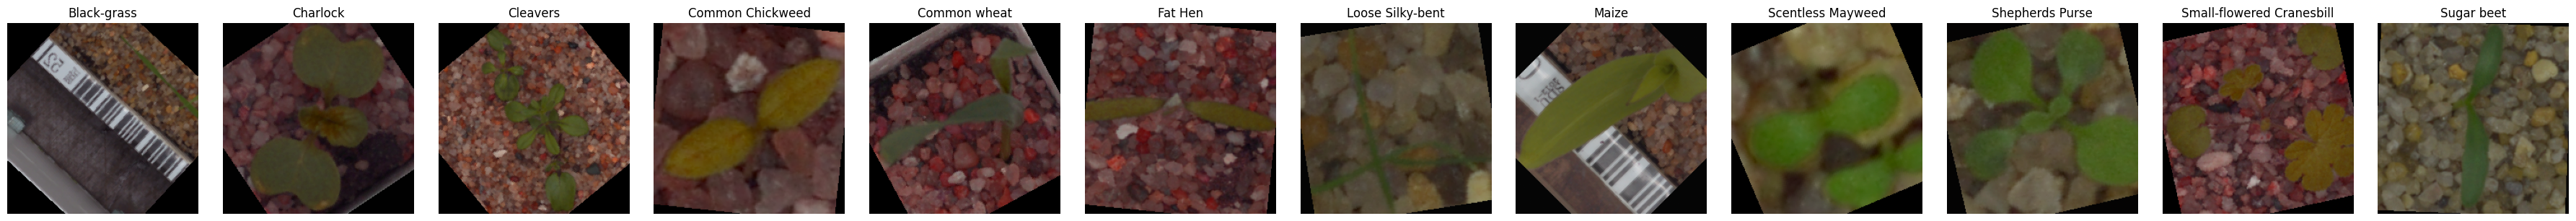
\includegraphics[width=0.9\textwidth]{../resources/sample_images.png}
            \caption{Example images of seedlings from the dataset}\label{fig:sample_images}
        \end{figure}
    \end{columns}
\end{frame}

\section{Problem Definition}
\begin{frame}{Problem Definition}
    \begin{columns}
        \column{0.5\textwidth}
        \begin{itemize}
            \item \textbf{Input:\\}Train set of \textit{4750} images of plant seedlings
            \item \textbf{Output:\\}Classification label for each image, indicating the species of each plant seedling
            \item \textbf{Goal:\\}High classification performance as measured by equation~\ref{eq:fscore}
            \item[] \cite{plant-seedlings-classification-evaluation,manning2009introduction,sokolova2009systematic,takahashi2022confidence}
        \end{itemize}
        \column{0.6\textwidth}
        \begin{equation}
            \text{Precision}_{\mu} = \frac{\sum_{i=1}^{C} \mathit{TP_i}}{\sum_{i=1}^{C} (\mathit{TP_i} + \mathit{FP_i})}\label{eq:precision}
        \end{equation}
        \begin{equation}
            \text{Recall}_{\mu} = \frac{\sum_{i=1}^{C}  \mathit{TP_i}}{\sum_{i=1}^{C} (\mathit{TP_i} + \mathit{FN_i})}\label{eq:recall}
        \end{equation}
        \begin{equation}
            \text{F1}_{\mu} = \frac{2 \times \text{Precision}_{\mu} \times \text{Recall}_{\mu}}{\text{Precision}_{\mu} + \text{Recall}_{\mu}}\label{eq:fscore}
        \end{equation}
    \end{columns}
\end{frame}

\section{Dataset}
\begin{frame}{Dataset}
    \begin{figure}
        \centering
        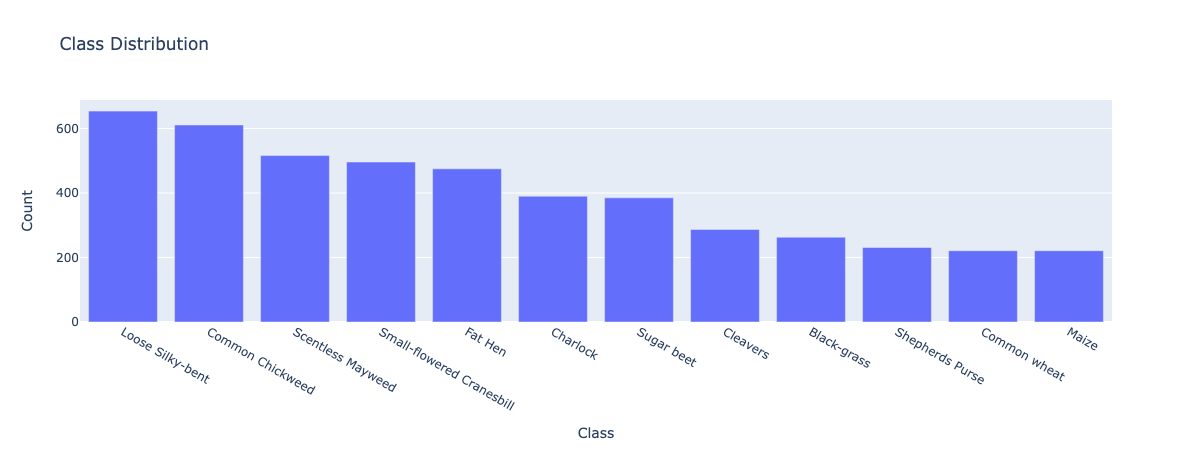
\includegraphics[width=0.9\textwidth]{../resources/class_distribution.png}
        \caption{Class distribution of the \textit{4750} training images}\label{fig:class-distribution}
    \end{figure}
\end{frame}

\section{Challenges}
\begin{frame}{Challenges}
    \begin{enumerate}
        \item \textbf{Inter-Class Similarity:\\}Certain seedlings can look strikingly similar
        \item \textbf{Intra-Class Variability:\\}Even within a single species, seedlings can vary significantly in appearance
        \item \textbf{Data Limitations:\\}With approximately \textit{960} unique plants, the dataset could be considered modest for training DL models
        \item \textbf{Model Architecture \& Capacity:\\}Choosing the right model architecture is crucial for effective feature extraction and classification
    \end{enumerate}
\end{frame}

\section{Model Architectures}
\begin{frame}{Overview}
    \begin{itemize}
        \item Explored three deep learning architectures for classification:
              \begin{itemize}
                  \item \textbf{Custom CNN:\\}Convolutional network built from scratch
                  \item \textbf{Pre-trained CNN:\\}ResNet-18~\cite{DBLP:journals/corr/HeZRS15}, pre-trained on ImageNet~\cite{5206848ImageNet}
                  \item \textbf{Pre-trained ViT:\\}vit\_base\_patch16\_224~\cite{Wightman_PyTorch_Image_Models}, pre-trained on ImageNet-21k~\cite{ridnik2021imagenet}
              \end{itemize}
        \item Also implemented ensemble combining predictions from all three architectures
        \item[] \vspace{0.5cm}
        \item \textbf{Aim:\\}Compare training from scratch vs. transfer learning and evaluate ensemble performance
    \end{itemize}
\end{frame}

\begin{frame}{Custom CNN (from scratch)}
    \begin{itemize}
        \item 5 convolutional layers with ReLU activations
        \item Filters gradually increase from \textit{16} to \textit{256}
        \item Max pooling layers after each conv layer
        \item 2 fully connected layers with dropout
        \item Final output layer with \textit{12} neurons (one for each class)
        \item Approximately \textit{2M} parameters
    \end{itemize}
\end{frame}

\begin{frame}{Pre-trained CNN (ResNet-18)}
    \begin{itemize}
        \item Pre-trained ResNet-18 model from torchvision
        \item Trained on ImageNet-1k dataset
        \item Final classification layer replaced with a new layer for \textit{12} classes
        \item Approximately \textit{11M} parameters
    \end{itemize}
\end{frame}

\begin{frame}{Pre-trained ViT (vit\_base\_patch16\_224)}
    \begin{itemize}
        \item Pre-trained vit\_base\_patch16\_224 model from timm library
        \item Trained on ImageNet-21k dataset
        \item Final classification layer replaced with a new layer for \textit{12} classes
        \item Weights frozen for all layers except the final classification layer
        \item Approximately \textit{86M} parameters, but only \textit{9,228} trainable parameters (due to frozen layers)
    \end{itemize}
\end{frame}

\begin{frame}{Ensemble}
    \begin{itemize}
        \item Combined predictions from all three models (Custom CNN, pre-trained CNN and pre-trained ViT)
        \item Used softmax probabilities from each model
        \item Weighted average of predictions based on test set performance
        \item[] \vspace{0.5cm}
        \item \textbf{Assumption:\\}Ensemble approaches often outperform single models~\cite{Stallkamp2012,DBLP:journals/corr/HeZRS15}
    \end{itemize}
\end{frame}

\begin{frame}{Summary}
    \begin{table}
        \caption{Model parameters and size of the custom CNN, pre-trained CNN and pre-trained ViT}
        \begin{center}
            \resizebox{0.9\linewidth}{!}{
                \begin{tabular}{|c|c|c|c|}
                    \hline
                    \textbf{Model}  & \textbf{Total Params} & \textbf{Trainable Params} & \textbf{Total Size (MB)} \\
                    \hline
                    Custom CNN      & 1,999,916             & 1,999,916                 & 34.91                    \\
                    \hline
                    Pre-trained CNN & 11,182,668            & 11,182,668                & 106.02                   \\
                    \hline
                    Pre-trained ViT & 85,655,820            & 9,228                     & 806.35                   \\
                    \hline
                \end{tabular}\label{tab:parameters}
            }
        \end{center}
    \end{table}
\end{frame}

\section{Training Strategies}
\begin{frame}{Optimization and Regularization I}
    \begin{itemize}
        \item \textbf{Optimizer:\\}Adam~\cite{kingma2017adammethodstochasticoptimization} with learning rate of \textit{0.001} and weight decay
        \item \textbf{Learning Rate Scheduler:\\}ReduceLROnPlateau reduced learning rate by \textit{50\%} if validation loss does not improve for \textit{2} epochs
    \end{itemize}
\end{frame}

\begin{frame}{Optimization and Regularization II}
    \begin{itemize}
        \item \textbf{Weight Decay:\\}L2 regularization with weight decay of \textit{0.0001}
        \item \textbf{Dropout:\\}Dropout layer with probability of \textit{0.5} after fully connected layer
        \item \textbf{Data Augmentation:\\}Random rotations, flips, and color jittering applied to training images
    \end{itemize}
\end{frame}

\begin{frame}{Data Augmentation}
    \begin{figure}
        \centering
        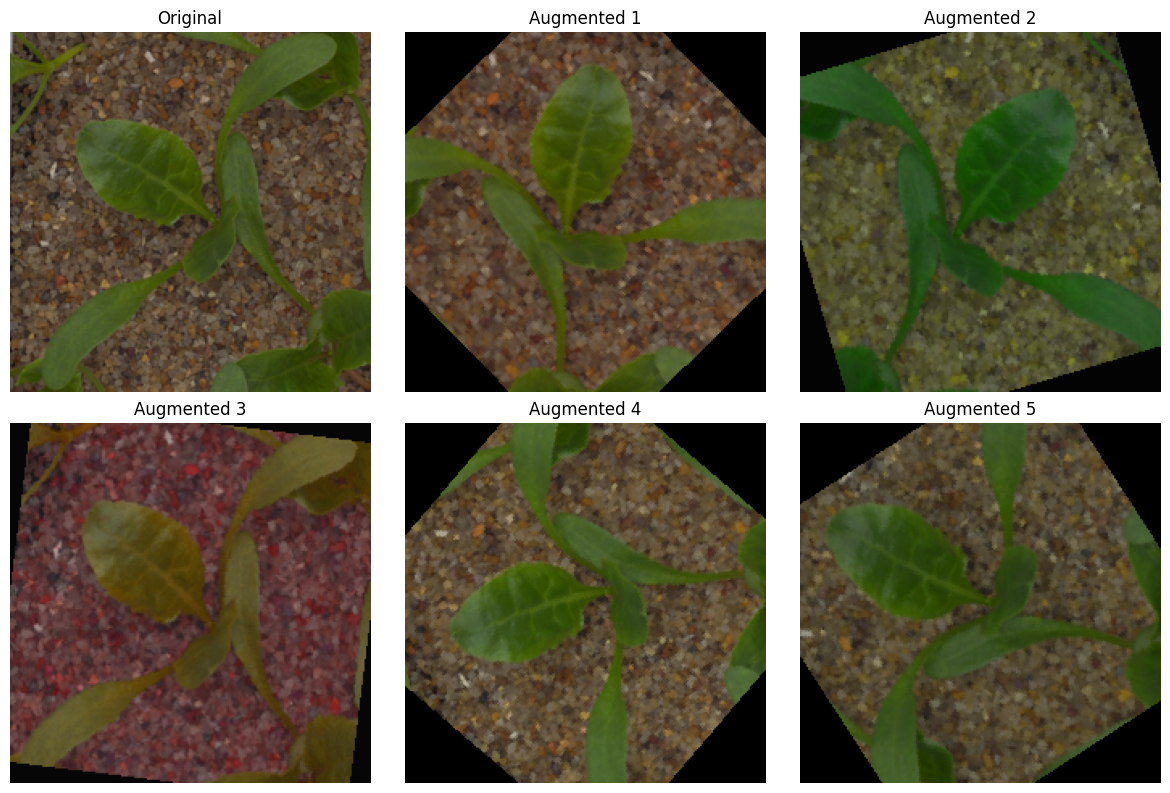
\includegraphics[width=0.9\textwidth]{../resources/data_augmentation.png}
        \caption{Original image (top left) and five augmented versions}\label{fig:data-augmentation}
    \end{figure}
\end{frame}

\section{Model Evaluation and Validation}
\begin{frame}{Validation Framework}
    \begin{itemize}
        \item Training and validation split of \textit{80\%} and \textit{20\%} respectively
        \item Training set: \textit{3800} images
        \item Validation set: \textit{950} images
        \item Kaggle challenge does not provide test set labels
        \item Validation set served as proxy for test set
        \item Early stopping based on validation loss (patience of \textit{10} epochs)
    \end{itemize}
\end{frame}

\begin{frame}{Training and Validation Losses I}
    \begin{figure}
        \centering
        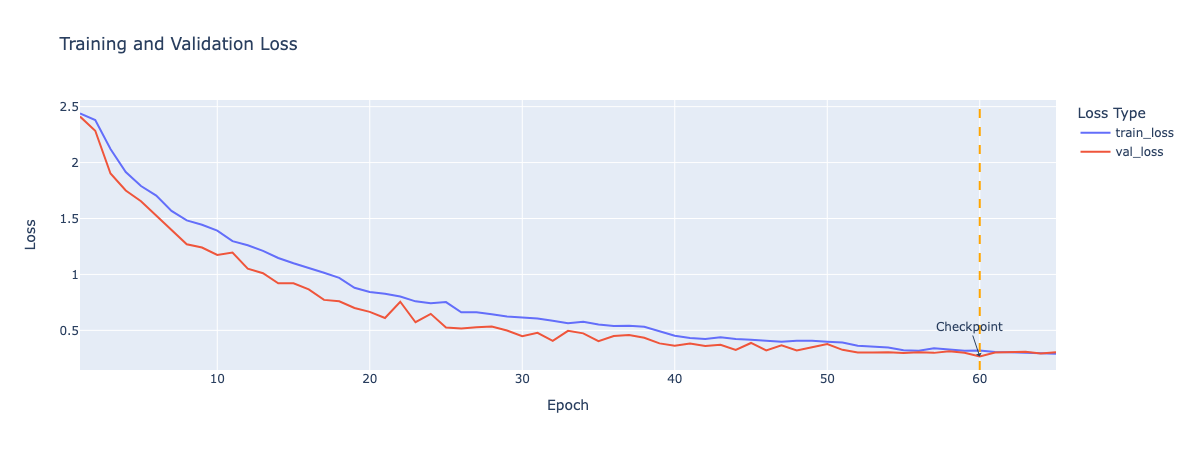
\includegraphics[width=0.9\textwidth]{../resources/custom_cnn/loss.png}
        \caption{Training and validation loss (custom CNN)}\label{fig:custom-cnn-loss}
    \end{figure}
    \begin{itemize}
        \item Gradual reduction in both losses
        \item Converged steadily around epoch \textit{60}
        \item Model could benefit from increased capacity
    \end{itemize}
\end{frame}

\begin{frame}{Training and Validation Losses II}
    \begin{figure}
        \centering
        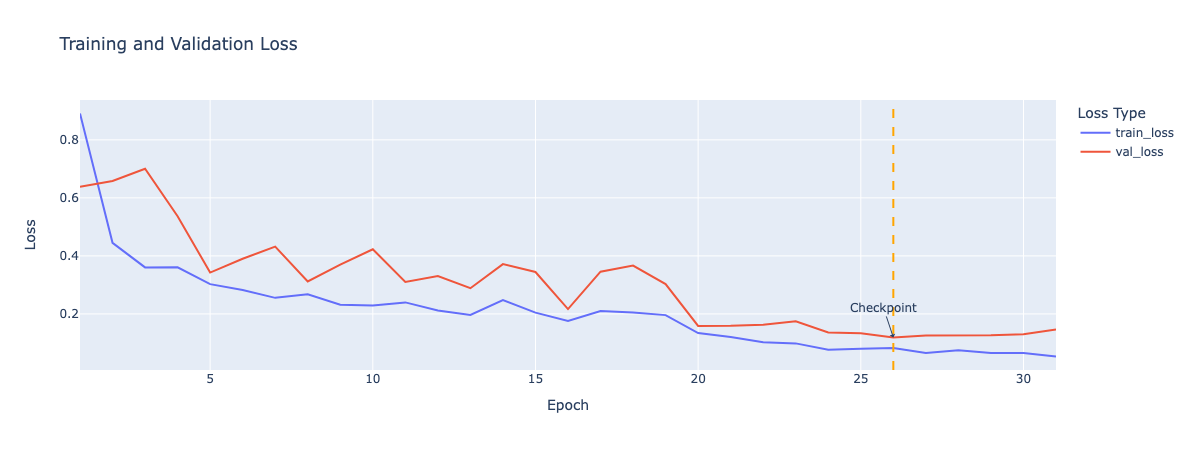
\includegraphics[width=0.9\textwidth]{../resources/resnet/loss.png}
        \caption{Training and validation loss (pre-trained CNN)}\label{fig:resnet-loss}
    \end{figure}
    \begin{itemize}
        \item Faster convergence compared to custom CNN
        \item Losses stabilized around epoch \textit{26}
        \item Began to clearly overfit after epoch \textit{30}
    \end{itemize}
\end{frame}

\begin{frame}{Training and Validation Losses III}
    \begin{figure}
        \centering
        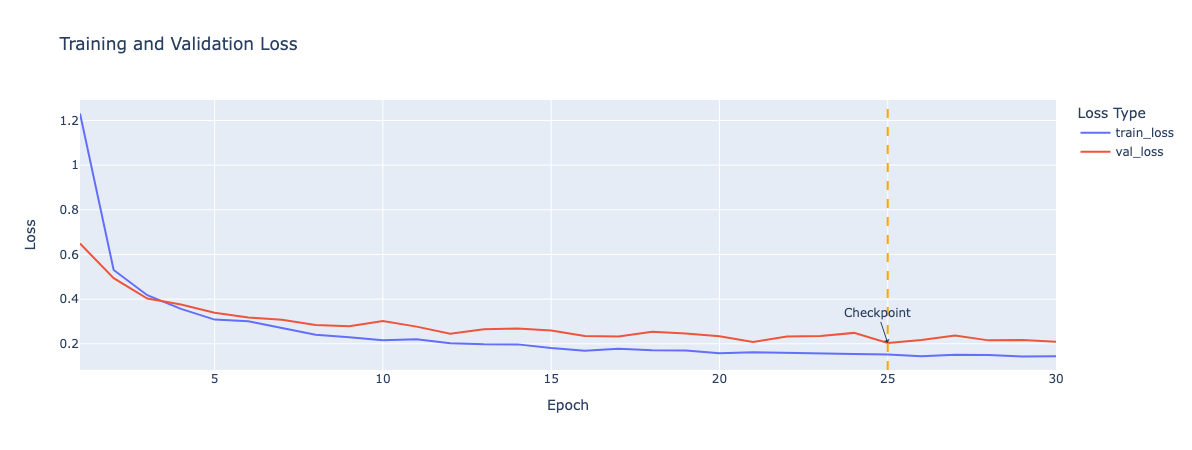
\includegraphics[width=0.9\textwidth]{../resources/vit/loss.png}
        \caption{Training and validation loss (pre-trained ViT)}\label{fig:vit-loss}
    \end{figure}
    \begin{itemize}
        \item Faster convergence compared to custom CNN
        \item Converged rapidly within \textit{25} epochs
        \item Could benefit from additional regularization to improve generalization
    \end{itemize}
\end{frame}

\section{Results and Analysis}
\begin{frame}{Quantitative Results}
    \begin{equation}
        \text{Accuracy} = \frac{\text{Number of Correct Predictions}}{\text{Total Number of Samples}}\label{eq:accuracy}
    \end{equation}
    \vspace{0.5cm}

    \begin{itemize}
        \item In addition to F1-score
        \item Simple and intuitive measure of performance
    \end{itemize}
\end{frame}

\begin{frame}{Quantitative Results}
    \begin{table}
        \caption{Quantitative results of the models on the train, validation and test set.}
        \begin{center}
            \resizebox{0.9\linewidth}{!}{
                \begin{tabular}{|c|c|c|c|c|c|}
                    \hline
                    \textbf{Model}    & \textbf{Train Loss} & \textbf{Val Loss} & \textbf{Val Accuracy} & \textbf{Test F1-Score} & \textbf{Epochs} \\
                    \hline
                    Guessing Baseline & -                   & -                 & -                     & 0.14105                & -               \\
                    \hline
                    Custom CNN        & 0.2897              & 0.3034            & 0.9042                & 0.92695                & 64              \\
                    \hline
                    Pre-trained CNN   & \textbf{0.0532}     & \textbf{0.1467}   & \textbf{0.9537}       & 0.96095                & 30              \\
                    \hline
                    Pre-trained ViT   & 0.1438              & 0.2089            & 0.9379                & \textbf{0.96725}       & 29              \\
                    \hline
                    \textbf{Ensemble} & -                   & -                 & -                     & \textbf{0.97103}       & -               \\
                    \hline
                \end{tabular}
                \label{tab:results}
            }
        \end{center}
    \end{table}
\end{frame}

\begin{frame}{Qualitative Results I}
    \begin{figure}
        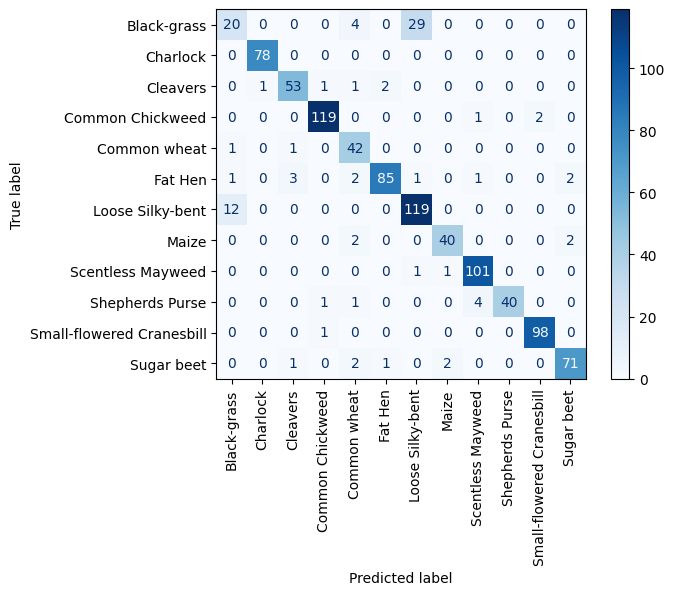
\includegraphics[width=0.6\linewidth]{../resources/custom_cnn/confusion.png}
        \caption{Confusion matrix~(custom CNN)}\label{fig:confusion-matrix-custom-cnn}
    \end{figure}
\end{frame}

\begin{frame}{Qualitative Results II}
    \begin{figure}
        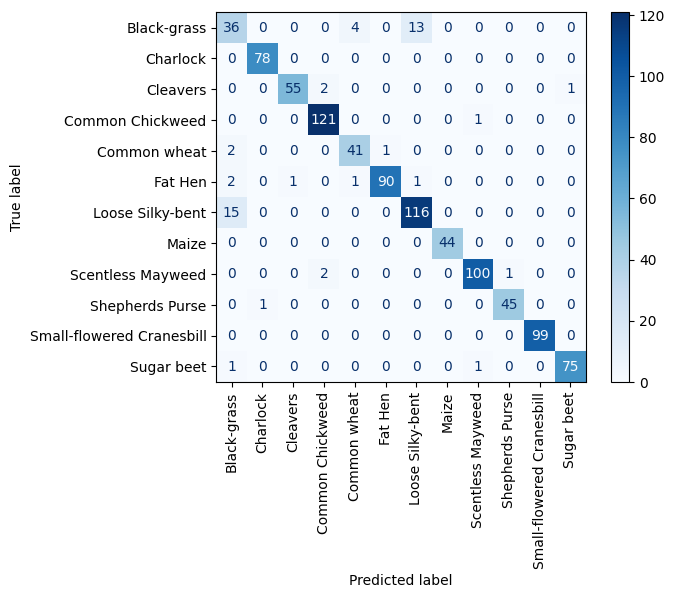
\includegraphics[width=0.6\linewidth]{../resources/resnet/confusion.png}
        \caption{Confusion matrix~(pre-trained CNN)}\label{fig:confusion-matrix-pretrained-cnn}
    \end{figure}
\end{frame}

\begin{frame}{Qualitative Results III}
    \begin{figure}
        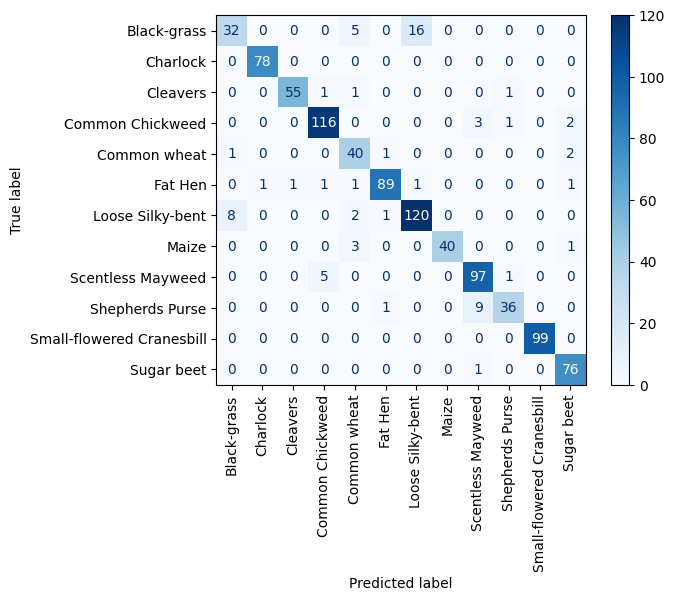
\includegraphics[width=0.6\linewidth]{../resources/vit/confusion.png}
        \caption{Confusion matrix~(pre-trained ViT)}\label{fig:confusion-matrix-pretrained-vit}
    \end{figure}
\end{frame}

\begin{frame}{Qualitative Results IV}
    \begin{itemize}
        \item Some misclassifications without a clear pattern
        \item Models struggled to distinguish between ``Loose Silky-bent'' and ``Black-grass''
    \end{itemize}
\end{frame}

\begin{frame}{Comparative Analysis}
    \begin{itemize}
        \item Ensemble model outperformed individual models
        \item Highest test F1-score of \textbf{0.97103}
        \item Pre-trained ViT achieved highest individual test F1-score of \textbf{0.96725}
        \item[] \vspace{0.5cm}
        \item Real-time inference was not required
        \item However, custom CNN is the lightest model and achieved a test F1-score of \textbf{0.92695}
    \end{itemize}
\end{frame}

\begin{frame}{Interpretability Measures}
    \begin{itemize}
        \item Pytorch-Grad-CAM library~\cite{jacobgilpytorchcam}
        \item Generates gradient-weighted class activation maps
        \item Provides insight into regions of the image that the model focuses on
        \item[] \vspace{0.5cm}
        \item Last two convolutional layers of the models were used to generate CAMs
    \end{itemize}
\end{frame}

\begin{frame}{Grad-CAM I}
    \begin{figure}
        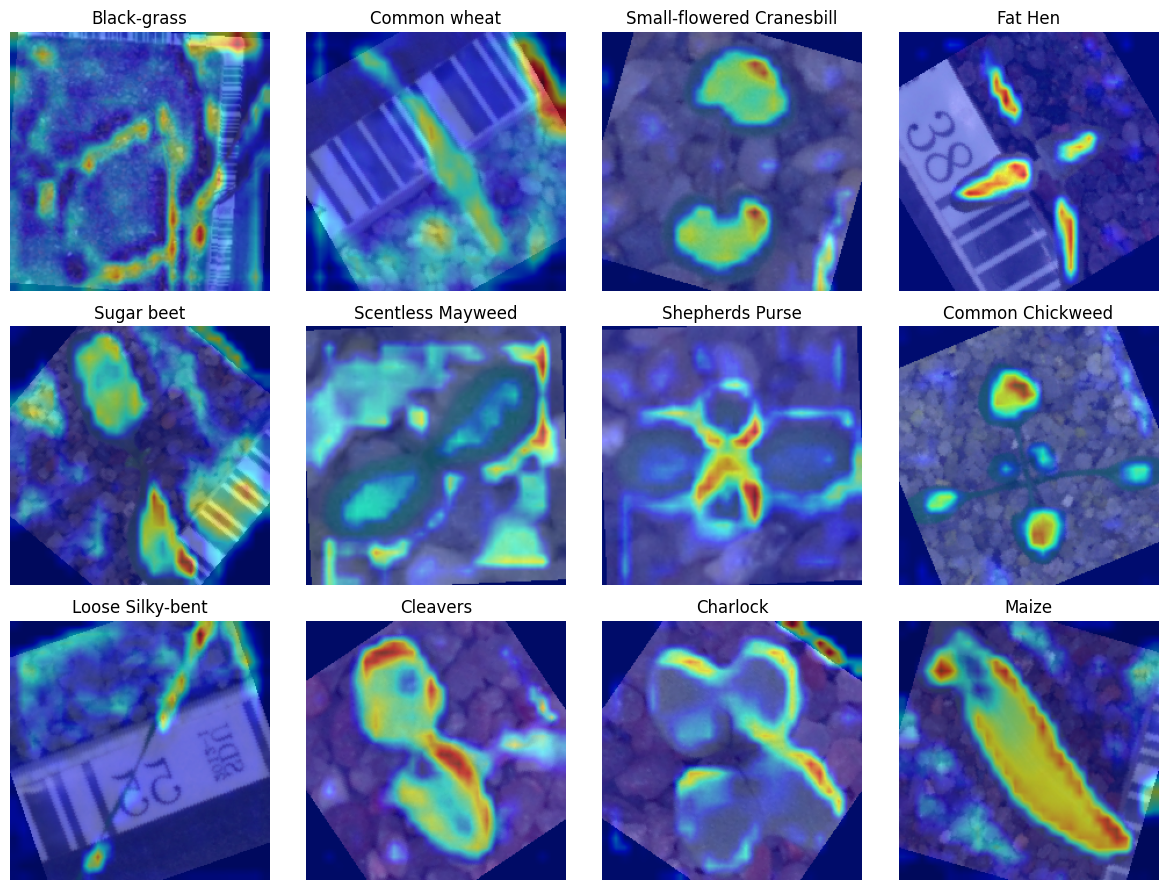
\includegraphics[width=0.4\linewidth]{../resources/custom_cnn/grad_cam.png}
        \caption{Grad-CAM (custom CNN)}\label{fig:grad-cam-custom-cnn}
    \end{figure}

    \begin{itemize}
        \item \textbf{Focused on the leaves for:\\}``Small-flowered Cranesbill'', ``Fat Hen'', ``Common Chickweed'', ``Cleavers'' and ``Maize''
        \item \textbf{Focused on the soil or background for:\\}``Black-grass'', ``Common wheat'', ``Sugar beet'', ``Scentsless Mayweed'' and ``Loose Silky-bent'
    \end{itemize}
\end{frame}

\begin{frame}{Grad-CAM II}
    \begin{figure}
        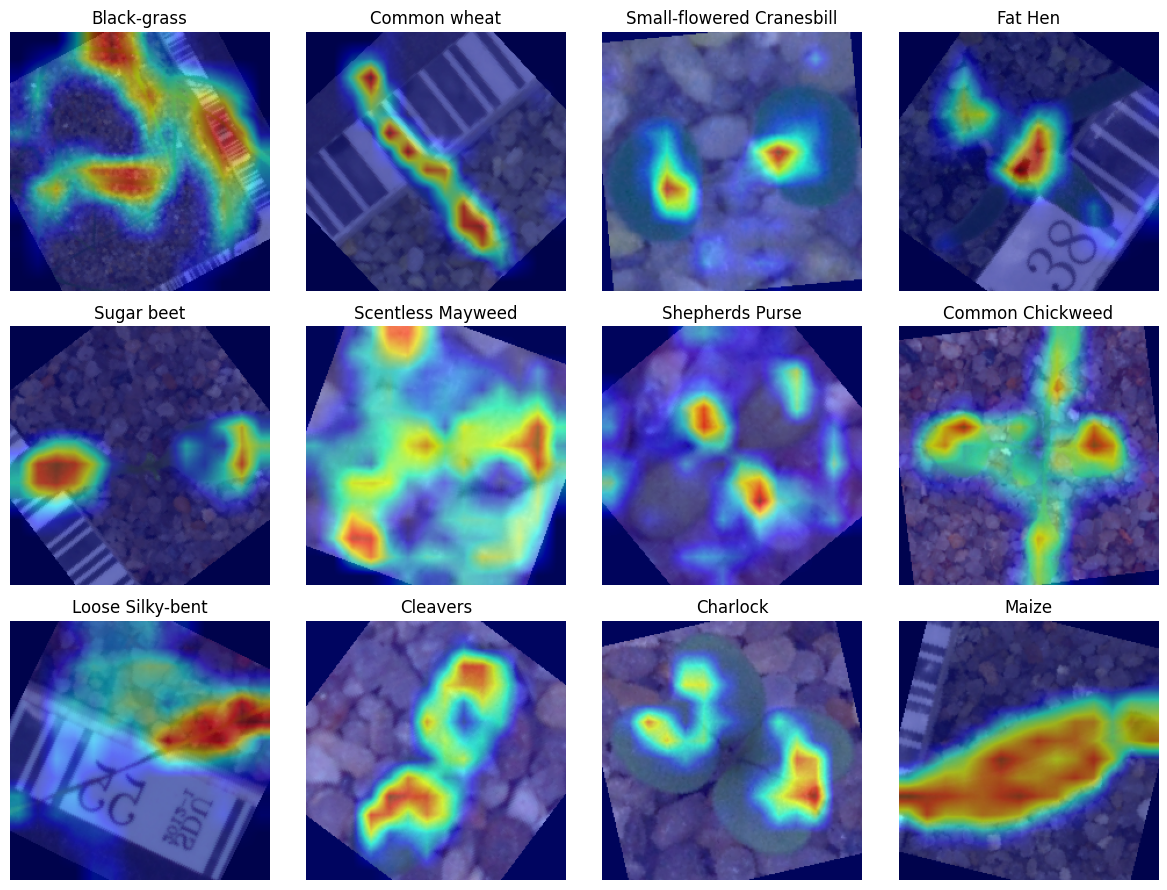
\includegraphics[width=0.4\linewidth]{../resources/resnet/grad_cam.png}
        \caption{Grad-CAM (pre-trained CNN)}\label{fig:grad-cam-pretrained-cnn}
    \end{figure}

    \begin{itemize}
        \item Focused more on the plants compared to the custom CNN
        \item Still background focus for ``Black-grass'', ``Scentsless Mayweed'' and ``Loose Silky-bent''
    \end{itemize}
\end{frame}

\begin{frame}{Grad-CAM III}
    \begin{figure}
        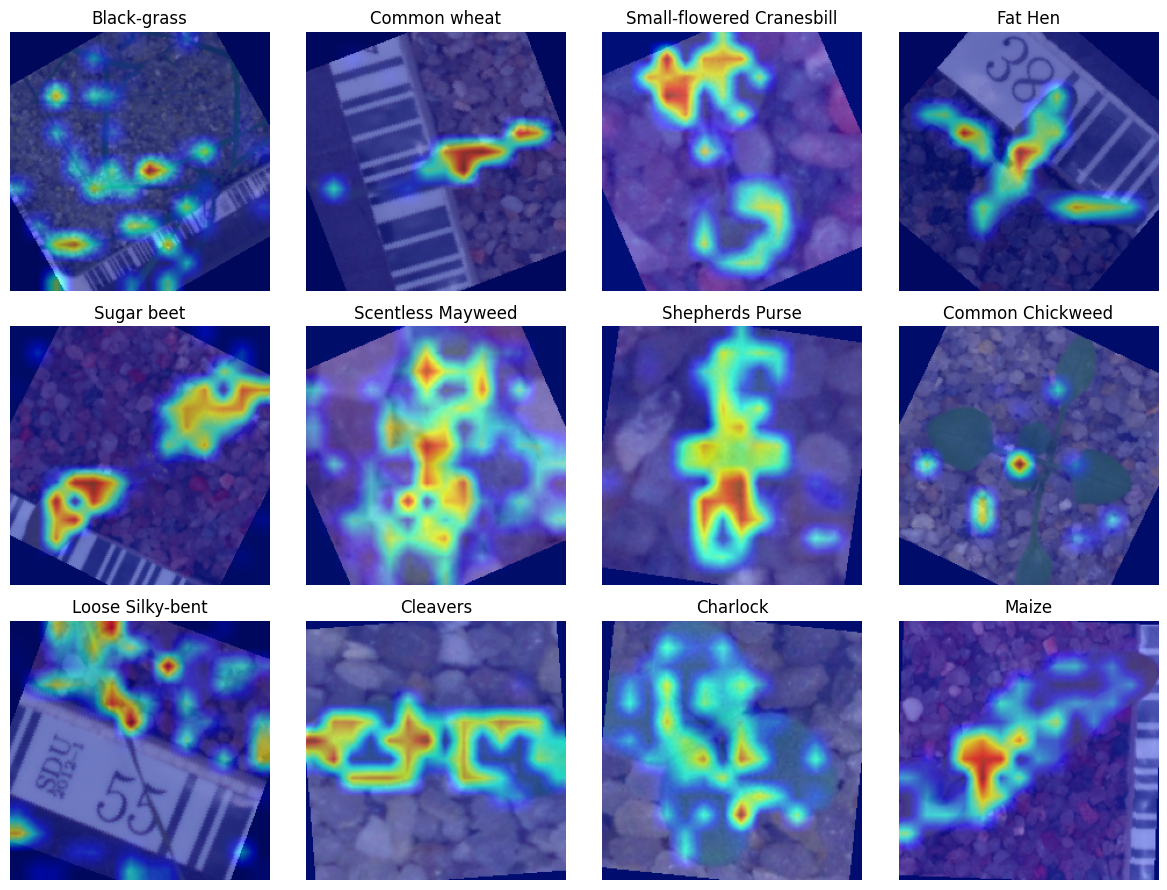
\includegraphics[width=0.4\linewidth]{../resources/vit/grad_cam.png}
        \caption{Grad-CAM (pre-trained ViT)}\label{fig:grad-cam-pretrained-vit}
    \end{figure}

    \begin{itemize}
        \item Same as pre-trained CNN
        \item Areas of interest look more \textit{blocky}
        \item Due to the nature of the ViT architecture (patch-based)
    \end{itemize}
\end{frame}

\section{Conclusion}
\begin{frame}{Conclusion I}
    \begin{itemize}
        \item Custom CNN achieved competitive performance
        \item Pre-trained models outperformed custom CNN\\(underscoring effectiveness of transfer learning)
        \item Ensemble model achieved the best performance\\(\textit{wisdom of the crowd}~\cite[Chapter~7]{geronoctober2022hands})
    \end{itemize}
\end{frame}

\begin{frame}{Conclusion II}
    \begin{itemize}
        \item Regularization techniques (data augmentation, dropout, weight decay) improved generalization
        \item Stratified training and validation split dealt with class imbalance (skewed dataset)
        \item ``Loose Silky-bent'' and ``Black-grass'' were consistently misclassified (high visual similarity)
        \item Frozen layers in ViT reduced trainable parameters
        \item Grad-CAM provided insight into model decision-making
    \end{itemize}
\end{frame}

\begin{frame}{Future Work}
    \begin{itemize}
        \item Add more models to the ensemble
        \item Train the ensemble on the validation set data to find the optimal weights for each model
        \item Explore deeper pre-trained networks\\(ResNet-50, DenseNet, EfficientNet)
        \item Collect additional labeled data or generate synthetic samples using GANs~\cite{goodfellow2014generativeadversarialnetworks}
        \item Image segmentation to remove background \textit{noise}
    \end{itemize}
\end{frame}

\begin{frame}[allowframebreaks, noframenumbering, plain]{References}
    \sloppy
    \printbibliography
\end{frame}

\begin{frame}
    \begin{center}
        \Huge
        \textbf{Thank you!}\\
        \vspace{1cm}
        \textit{Questions?}
    \end{center}
\end{frame}

\end{document}